\documentclass{article}
\usepackage[T1]{fontenc}
\usepackage{lmodern}
\usepackage{graphicx}
\usepackage{amsmath,amssymb}
\usepackage[a4paper,margin=2cm]{geometry}
\usepackage[absolute,overlay]{textpos}
\setlength{\TPHorizModule}{1mm}
\setlength{\TPVertModule}{1mm}
\usepackage[indonesian]{babel}
\usepackage{hyperref}
\setlength{\emergencystretch}{2em}
% unit: Halaman 15

\begin{document}

% === Halaman 15 (llm) ===

(b) $P + (-P) = O$, di sini $O$ adalah titik di $infinity$

\vspace{10mm}

$P' = -P$ adalah elemen invers:
\[ P + P' = P + (-P) = O \]

$O$ adalah elemen netral:
\[ P + O = O + P = P \]

\vspace{20mm}

\centering{\textcolor{red}{Sumber gambar: Andreas Steffen, Elliptic Curve Cryptography}}

% deskripsi: Grafik kurva eliptik pada koordinat Kartesius yang menunjukkan titik P dan inversnya -P, dengan garis bantu vertikal berwarna hijau yang melewati kedua titik tersebut.
% bbox normalisasi: [0.4740, 0.2030, 0.8440, 0.8170]
\begin{textblock*}{77.70mm}(99.54mm,60.29mm)
\noindent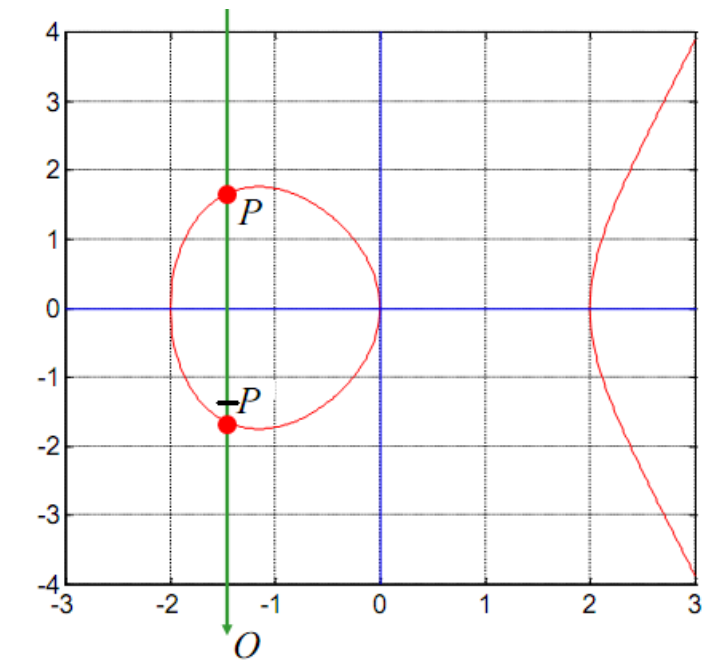
\includegraphics[width=77.70mm,height=182.36mm]{../../images/llm/page_015_img_01.png}%
\end{textblock*}

\end{document}
